\chapter{Introducción}
\thispagestyle{empty}

\section{Definición del problema}
%En este apartado expondremos un poco el contexto de la identificación facial (contextualizándola, seguramente, dentro de la identificación humana forense.) y cómo se relaciona con la distancia cámara-sujeto y la distorsión de perspectiva (explicar un poco qué son), las principales limitaciones y factores determinantes del reconocimiento automático, y una breve descripción de para qué sirve conocer la distancia cámara-sujeto. Por último definiremos el problema que vamos a abordar en el TFG.

% Muy importante que seas muy visual en tus explicaciones. No dudes en crear figuras que sirvan de apoyo al texto (incluyendo siempre captions informativas, y enlazando y referenciando las figuras adecuadamente en el cuerpo del texto). Por ejemplo, para explicar lo que es la SCD y la distorsión de perspectiva. 

Durante la última década, la identificación facial ha ganado una relevancia significativa gracias a la revolución del aprendizaje profundo y los sistemas automáticos de reconocimiento facial. Este avance ha conducido a una expansión de las posibles aplicaciones en el mercado actual desde los campos del cumplimiento de la ley o la ciencia forense, hasta áreas del sector privado como el comercio minorista, las aplicaciones multimedia o la seguridad. Además, el desarrollo tecnológico en el ámbito de la imagen ha mejorado tanto la calidad como la disponibilidad de datos fotográficos, lo cual facilita un análisis más exhaustivo de los factores que influyen en las imágenes fotográficas.

Las técnicas de identificación facial normalmente son realizadas por expertos con o sin la ayuda de sistemas automáticos. Los expertos analizan los datos y evalúan las características anatómicas de un individuo desconocido para compararlas con las de uno o varios individuos conocidos. Actualmente existen cuatro métodos de comparación facial reconocidos: análisis morfológico, superposición, foto-antropometría y comparación holística~\cite{3}.

Para que este análisis sea confiable y concluyente, los datos (fotografías faciales), deben estar en unas condiciones adecuadas (calidad, resolución, enfoque o iluminación) y la escena (punto de vista de la cámara, pose de la cabeza, expresión facial) debe ser lo más neutral y representativa posible~\cite{1,2}. Estos requisitos nos aseguran que los rasgos faciales sean lo más fieles posible a las características anatómicas del individuo, y por tanto, permiten que las técnicas de identificación sean más robustas.

Muchos estudios han identificado limitaciones en los actuales métodos de reconocimiento facial automático. Los principales factores desafiantes son la pose, la iluminación, la expresión y la variación en la edad~\cite{4,6}. Sin embargo también existen otros factores importantes como la oclusión, el género o la etnia~\cite{5,7}.

Uno de los factores más importantes en las fotografías faciales es la distorsión de perspectiva, la cual puede provocar deformaciones en los rasgos faciales, como en las orejas, la nariz o la forma general del rostro, especialmente cuando la cámara está muy cerca del sujeto al momento de tomar la fotografía~\cite{12} (ver Figura~\ref{fig1.1}). Esta alteración en la perspectiva repercute negativamente en los sistemas de reconocimiento automático~\cite{9,10,11}, lo cual puede obstaculizar la identificación precisa de individuos. 

\begin{figure}[h]
	\centering
	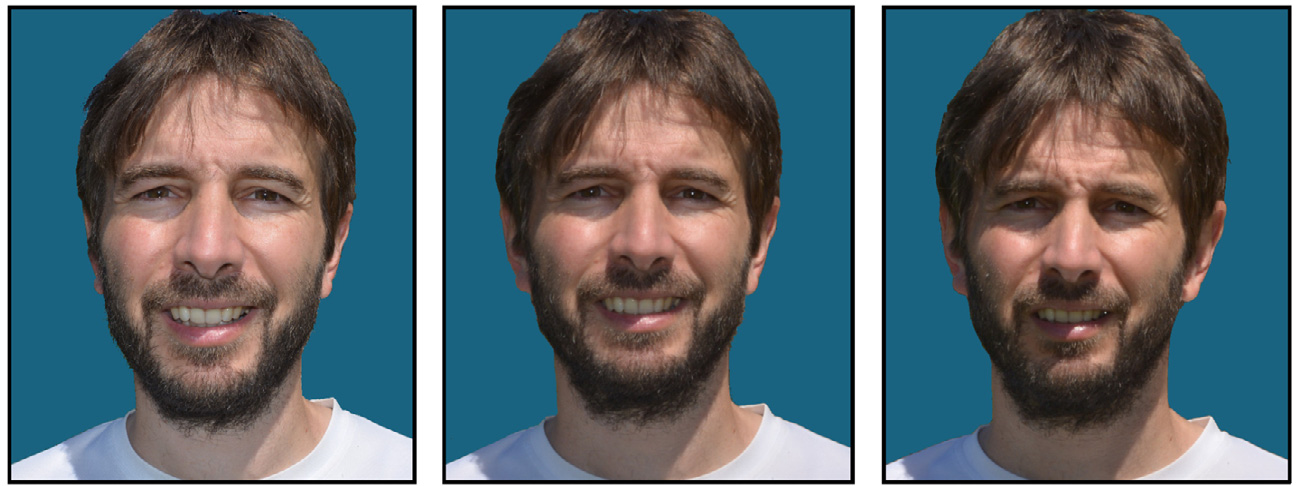
\includegraphics[scale=0.25]{imagenes/cap1/facial_distortion.png}
	\caption{Efectos de la distorsión de perspectiva en características faciales de fotografías realizadas a diferentes SCD: 0.5 m, 1 m y 3 m. Estos efectos varían en relación a la distancia y son independientes de la longitud focal~\cite{14}}
	\label{fig1.1}
\end{figure}

%-----------

La distorsión de perspectiva está estrechamente relacionada con la distancia cámara-sujeto (subject-to-camera distance, SCD en adelante), de hecho, la relación es de decremento logarítmico, es decir, valores pequeños de la SCD corresponden con una mayor distorsión, mientras que la distorsión disminuye conforme la SCD aumenta~\cite{23}. Conocer la SCD en fotografías faciales permite cuantificar la cantidad de distorsión presente en la imagen, así como las diferencias en la distorsión entre dos conjuntos de imágenes. Esta información es útil para reproducir con fiabilidad las condiciones originales de una escena, especialmente en el ámbito forense, y para facilitar el desarrollo de técnicas que permitan la corrección precisa de dicha distorsión

% explicación un poco de la longitud focal y tamaño del sensor?
La SCD, a diferencia de otros parámetros de la cámara como la longitud focal o el tamaño del sensor, no puede obtenerse directamente desde los metadatos de la fotografía~\cite{8}. Por tanto, se necesita un método preciso para su estimación. 

%\begin{figure}[h]
%	\centering
%	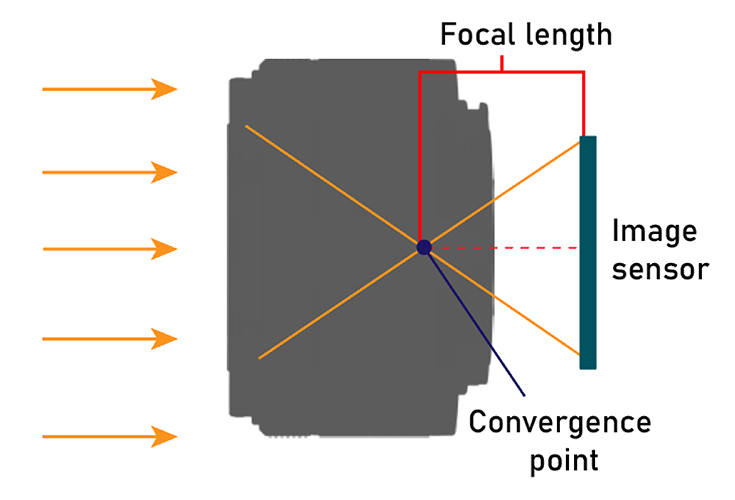
\includegraphics[scale=1]{imagenes/cap1/focal_lenght.jpg}
%	\caption{Parámetros de la cámara: longitud focal y sensor}
%	\label{fig1.2}
%\end{figure}

% el final podría estar mejor explicado porque no se entiende mucho lo de las longitudes focales
En los últimos años se han utilizado varios métodos que combinan técnicas manuales y automatizadas basadas en puntos de referencia o en características anatómicas de la cara\cite{28,30}. Sin embargo, no se han obtenido resultados favorables debido a la dificultad para obtener estimaciones precisas en largas distancias por la diversa fisionomía de la cara, y a los problemas relacionados con los parámetros de la cámara, como el recorte de imágenes o la combinación de diferentes longitudes focales en el mismo conjunto de datos.

El único método totalmente automatizado para estimar la SCD en fotografías faciales, hasta la fecha, se conoce como FacialSCDnet~\cite{14}. Este método utiliza una arquitectura basada en aprendizaje profundo para procesar fotografías faciales y estimar la SCD con precisión. Sin embargo, las soluciones basadas en aprendizaje profundo tienen sesgos sobre los datos y las muestras deben ser lo más representativas posible. 

Considerando todos estos aspectos, el presente Trabajo de Fin de Grado (TFG) consiste en mejorar el método actual del estado del arte en la estimación automática de la distancia cámara-sujeto en fotografías faciales mediante el uso de técnicas de aprendizaje profundo.


\section{Motivación}
%Motivación: listar diferentes ámbitos de aplicación por los que la información de distancia puede ser útil.
%Ejemplo: En reconocimiento facial y biometría, la calidad de una fotografía es muy importante. Saber la SCD permitiría conocer si las proporciones de la cara en la fotografía se ajustan a la anatomía real o están distorsionadas.
% También estaría bien enfocar el problema en que las soluciones deep learning tienen sesgos sobre los datos y las muestras tienen que ser representativas. Así justificamos que sea una evolución de un trabajo anterior.

% Hay que mejorar la redacción
En el ámbito forense, el principal foco recae sobre la determinación de la identidad humana cuando se dispone de información esquelética~\cite{15}. En las últimas décadas, los antropólogos han centrado su atención en mejorar las técnicas para realizar una identificación más precisa. En este contexto, la estimación de la SCD juega un papel crucial, ya que, si estimamos la SCD con fiabilidad, podemos recrear la imagen con los restos esqueléticos (aplicando el valor de la SCD) \cite{21}. A continuación, realizamos las comparaciones anatómicas mediante la superposición craneofacial~\cite{22} para identificar si se corresponde con la misma persona (ver Figura~\ref{fig2}). Si los parámetros de adquisición entre ambas imágenes (normal y esquelética) son distintos entonces dificultaría el análisis morfológico~\cite{13}.

\begin{figure}[h]
	\centering
	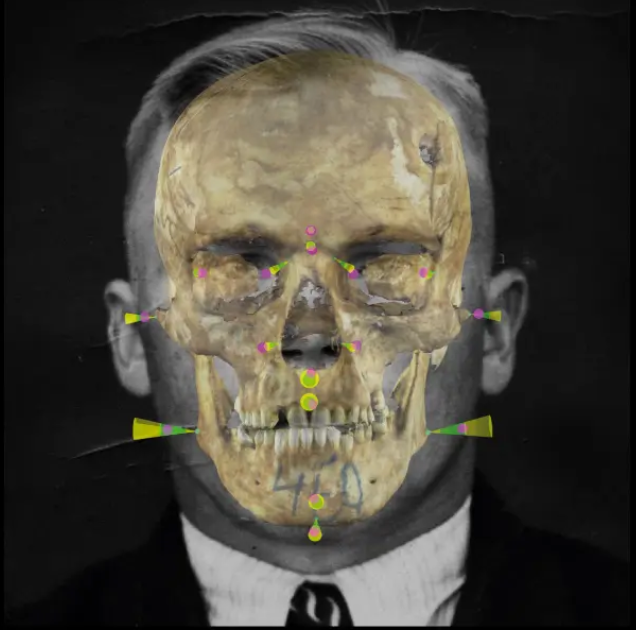
\includegraphics[scale=0.25]{imagenes/cap1/skull_superimposition.png}
	\caption{Ejemplo de superposición craneofacial~\cite{23}.}
	\label{fig2}
\end{figure}

% Aquí hablar sobre reconocimiento facial y biometría para saber si una imagen se adapta a la realidad o está distorsionada, incluso aplicar técnicas para mitigar la distorsión
En el ámbito de la biometría y el reconocimiento facial, conocer la SCD es fundamental para comprender y corregir las distorsiones de perspectiva que pueden afectar a la precisión de la identificación. Esta distancia influye directamente en la representación facial capturada, afectando la geometría y proporciones del rostro (ver Figura \ref{fig2.1}). Un entendimiento preciso de esta medida permite aplicar técnicas de corrección de distorsión~\cite{16,17} para garantizar una representación fiel y coherente de las características faciales, mejorando de esta manera la precisión y fiabilidad de los sistemas biométricos y de reconocimiento facial.
% Por otro lado, en el ámbito del reconocimiento facial y la biometría, la SCD desempeña un papel crucial en este proceso. Esta medida proporciona información sobre si las proporciones faciales capturadas en la fotografía coinciden con la anatomía real del individuo o si han sido distorsionadas (ver Figura \ref{fig2.1}). Conocer la SCD nos permite aplicar técnicas de correción de distorsión~\cite{16,17}.

\begin{figure}[h]
	\centering
	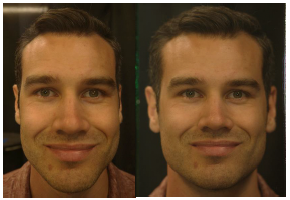
\includegraphics[scale=1]{imagenes/cap1/dist-nodist.png}
	\caption{A la izquierda la fotografía distorsionada, a la derecha la fotografía sin distorsión~\cite{17}.}
	\label{fig2.1}
\end{figure}


% Aquí hablar sobre mejora de actual estado del arte por sesgos en los datos pero más detallado
En el campo del aprendizaje profundo, es común encontrar sesgos \cite{39} en los datos que pueden afectar a la precisión y generalización de las soluciones. Dichos sesgos pueden surgir de diversos factores, como la falta de diversidad o el ruido excesivo en el conjunto de datos utilizado para entrenar los modelos. Esto también ocurre en los métodos actuales para la estimación automática de la SCD. Es por ello que, una forma de mejorar el conjunto de datos podría ser incluir una variedad más amplia de grupos étnicos, edades, géneros, expresiones faciales, condiciones de iluminación y fondos, así como modelos tanto faciales como de cuerpo completo.
Al hacerlo, se busca mitigar los sesgos inherentes a los datos y desarrollar modelos más robustos y equitativos. Esta mejora implica una mayor capacidad de generalización y adaptación a una amplia gama de situaciones y contextos.

Por todo ello, la estimación de la SCD de forma precisa y generalizable tiene el potencial de impulsar avances significativos en diversos campos de investigación.


\section{Objetivos}
% Cambiar esto
%El objetivo general de este TFG consiste en mejorar el método actual del estado del arte en la estimación automática de la distancia cámara-sujeto en fotografías faciales.
 El objetivo general de este TFG consiste en desarrollar un modelo de aprendizaje profundo adecuado para mejorar la estimación de la distancia cámara-sujeto en fotografías faciales. Para el desarrollo del proyecto, dividiremos el objetivo general en una serie de objetivos parciales:
\begin{enumerate}
    \item Realizar un análisis exhaustivo del estado del arte para la estimación de la SCD en fotografías faciales.
    \item Generar un conjunto de datos sintético de mayor calidad (utilizando modelos 3D más completos de cuerpo entero y poses distintas, con fondos e iluminación más realistas).
    \item Realizar un estudio experimental que permita validar los enfoques propuestos y extraer conclusiones sobre su aplicabilidad al problema.
    \item Desarrollar y entrenar con nuevas arquitecturas que mejoren los resultados.
    \item Usar tecnologías más recientes que mejoren los tiempos de aprendizaje y los resultados obtenidos.
\end{enumerate}

\section{Planificación del proyecto}

Para abordar el desarrollo de este proyecto, es esencial considerar que el TFG tiene asignados 12 créditos ECTS, lo que equivale a aproximadamente 300 horas de trabajo. Dada la distribución temporal del segundo cuatrimestre, con unas 20 semanas disponibles, se estima que se requerirá dedicar al TFG unas 20 horas semanales, equivalentes a 4 horas diarias durante 5 días a la semana. Se reservan así 4 semanas como margen para posibles retrasos o imprevistos que puedan surgir durante el desarrollo del proyecto.

En cuanto a la metodología de desarrollo, se ha optado por seguir un enfoque basado en el ciclo de vida en cascada~\cite{38}, aunque con una variante que permite retroalimentación. Aunque el proyecto presenta requisitos y objetivos claros, se reconoce la posibilidad de ajustes menores durante su desarrollo, especialmente a medida que se obtenga más información sobre el problema y los métodos. Esta flexibilidad se considera crucial para adaptarse a posibles cambios en el contexto o los requisitos del proyecto.

Las fases del ciclo de vida del proyecto son las siguientes:

A continuación se describen las fases del ciclo de vida del proyecto:
\begin{itemize}
	\item Análisis de Requisitos: Consiste en las reuniones iniciales con los clientes, en este caso los directores del TFG. Se realiza un análisis del problema y un estudio detallado de la bibliografía existente
	\item Diseño: Consiste en la exploración y selección de los métodos apropiados basados en el análisis previo, tanto para la resolución como para la validación de la solución propuesta. Además, se llevarán a cabo pruebas preliminares y se elaborará el diseño del software experimental.
	\item Implementación: Consiste en la adaptación del código de los modelos investigados, la implementación de nuevas funcionalidades y la generación de un conjunto de datos sintético junto con su posterior preprocesado.
	\item Pruebas: Consiste en la realización de diversos experimentos para validar el funcionamiento del software desarrollado, utilizando los modelos y datos previamente definidos.
\end{itemize}

\begin{table}[htbp]
	\resizebox{\textwidth}{!}{%
	\begin{tabular}{|c|c|*{4}{c}|*{4}{c}|*{5}{c}|*{4}{c}|*{3}{c}|}
	\hline
	\rowcolor[HTML]{FFC702} 
	\cellcolor[HTML]{FFC702} & \cellcolor[HTML]{FFC702} & \multicolumn{4}{c|}{\cellcolor[HTML]{FFC702}Febrero} & \multicolumn{4}{c|}{\cellcolor[HTML]{FFC702}Marzo} & \multicolumn{5}{c|}{\cellcolor[HTML]{FFC702}Abril} & \multicolumn{4}{c|}{\cellcolor[HTML]{FFC702}Mayo} & \multicolumn{3}{c|}{\cellcolor[HTML]{FFC702}Junio} \\
	\rowcolor[HTML]{FFC702} 
	\multirow{-2}{*}{\cellcolor[HTML]{FFC702}Tarea} & \multirow{-2}{*}{\cellcolor[HTML]{FFC702}\begin{tabular}[c]{@{}c@{}}Semanas\\ - Horas\end{tabular}} & 5 & 12 & 19 & 26 & 4 & 11 & 18 & 25 & 1 & 8 & 15 & 22 & 29 & 6 & 13 & 20 & 27 & 3 & 10 & 17 \\ \hline
	Análisis de Requisitos & 3 - 60 & \cellcolor[HTML]{9B9B9B} & \cellcolor[HTML]{9B9B9B} & \cellcolor[HTML]{9B9B9B} &  &  &  &  &  &  &  &  &  &  &  &  &  &  &  &  &  \\ \cline{1-1}
	Diseño & 3 - 60 &  &  &  & \cellcolor[HTML]{9B9B9B}{\color[HTML]{C0C0C0} } & \cellcolor[HTML]{9B9B9B}{\color[HTML]{C0C0C0} } & \cellcolor[HTML]{9B9B9B}{\color[HTML]{C0C0C0} } &  &  &  &  &  &  &  &  &  &  &  &  &  &  \\ \cline{1-1}
	Implementación & 5 - 90 &  &  &  &  &  &  & \cellcolor[HTML]{9B9B9B} & \cellcolor[HTML]{9B9B9B} & \cellcolor[HTML]{9B9B9B} & \cellcolor[HTML]{9B9B9B} & \cellcolor[HTML]{9B9B9B} &  &  &  &  &  &  &  &  &  \\ \cline{1-1}
	Pruebas & 5 - 90 &  &  &  &  &  &  &  &  &  &  &  & \cellcolor[HTML]{9B9B9B} & \cellcolor[HTML]{9B9B9B} & \cellcolor[HTML]{9B9B9B} & \cellcolor[HTML]{9B9B9B} & \cellcolor[HTML]{9B9B9B} &  &  &  &  \\ \hline
	\end{tabular}%
	}
	\caption{Planificación inicial del proyecto}
	\label{planif-ini}
\end{table}